% !TEX TS-program = xelatex
% !TEX encoding = UTF-8 Unicode

% \documentclass[AutoFakeBold]{LZUThesis}
\documentclass[AutoFakeBold]{LZUThesis}
  
  \usepackage{wasysym}
  \usepackage{enumitem}
  \usepackage[most]{tcolorbox}
  \usepackage{multirow}
  \usepackage{inputenc}
  \usepackage{tikz}
  \usepackage{bbding}
  \usetikzlibrary{arrows.meta, decorations.markings}
  \usepackage{hyperref}
  \usepackage[numbers,sort&compress]{natbib}
  \usepackage{pdfpages}
  % \newcommand{\upcite}[1]{\textsuperscript{\textsuperscript{\cite{#1}}}}
  \allowdisplaybreaks[4]
  \usepackage{pdfpages}
  \usepackage[many]{tcolorbox}
  \usepackage{setspace}
  % \setmonofont{MapleMono-NF-CN-Medium}
  \setmonofont{MapleMono-NF-CN-Regular}
  
  % \newtcolorbox[auto counter, number within=section, list inside=listoftables]{fancybox}[2][]{
  \newcommand{\supercite}[1]{\textsuperscript{\textsuperscript{\cite{#1}}}}
  \newtcolorbox[use counter=table]{fancybox}[2][]{
      title=Code~\thetcbcounter: #2,
      breakable, left=1cm,
      label={code:#2},
      % list entry=code~\thetcbcounter: #2
      % colback=yellow!10!white, colframe=red!50!black
  }
  
  
  
  
  
  
  
  
  \usepackage[dvipsnames]{xcolor}
  \usepackage{tikz}
  \usetikzlibrary{backgrounds}
  \usetikzlibrary{arrows,shapes}
  \usetikzlibrary{tikzmark}
  \usetikzlibrary{calc}
  
  \usepackage{amsmath}
  \usepackage{amsthm}
  \usepackage{amssymb}
  \usepackage{mathtools, nccmath}
  \usepackage{wrapfig}
  \usepackage{comment}
  \usepackage{subfigure}
  
  % To generate dummy text
  \usepackage{blindtext}
  
  
  %color
  %\usepackage[dvipsnames]{xcolor}
  % \usepackage{xcolor}
  
  
  %\usepackage[pdftex]{graphicx}
  \usepackage{graphicx}
  % declare the path(s) for graphic files
  %\graphicspath{{../Figures/}}
  
  % extensions so you won't have to specify these with
  % every instance of \includegraphics
  % \DeclareGraphicsExtensions{.pdf,.jpeg,.png}
  
  % for custom commands
  \usepackage{xspace}
  
  % table alignment
  \usepackage{array}
  \usepackage{ragged2e}
  \newcolumntype{P}[1]{>{\RaggedRight\hspace{0pt}}p{#1}}
  \newcolumntype{X}[1]{>{\RaggedRight\hspace*{0pt}}p{#1}}
  
  % color box
  \usepackage{tcolorbox}
  
  
  % for tikz
  \usepackage{tikz}
  %\usetikzlibrary{trees}
  \usetikzlibrary{arrows,shapes,positioning,shadows,trees,mindmap}
  % \usepackage{forest}
  \usepackage[edges]{forest}
  \usetikzlibrary{arrows.meta}
  \colorlet{linecol}{black!75}
  \usepackage{xkcdcolors} % xkcd colors
  
  
  % for colorful equation
  \usepackage{tikz}
  \usetikzlibrary{backgrounds}
  \usetikzlibrary{arrows,shapes}
  \usetikzlibrary{tikzmark}
  \usetikzlibrary{calc}
  % Commands for Highlighting text -- non tikz method
  \newcommand{\highlight}[2]{\colorbox{#1!17}{$\displaystyle #2$}}
  %\newcommand{\highlight}[2]{\colorbox{#1!17}{$#2$}}
  \newcommand{\highlightdark}[2]{\colorbox{#1!47}{$\displaystyle #2$}}
  
  % my custom colors for shading
  \colorlet{mhpurple}{Plum!80}
  
  
  % Commands for Highlighting text -- non tikz method
  \renewcommand{\highlight}[2]{\colorbox{#1!17}{#2}}
  \renewcommand{\highlightdark}[2]{\colorbox{#1!47}{#2}}
  
  % Some math definitions
  \newcommand{\lap}{\mathrm{Lap}}
  \newcommand{\pr}{\mathrm{Pr}}
  
  \newcommand{\Tset}{\mathcal{T}}
  \newcommand{\Dset}{\mathcal{D}}
  \newcommand{\Rbound}{\widetilde{\mathcal{R}}}
  
  
  
  
  \newcommand{\code}[1]{\lstinline|#1|}





\begin{document}

\title{{组织蛋白酶家族对于}{体内屏障衰老的作用与机制}}

\entitle{{Cathepsin Family: Mechanisms and Impact}{on Aging of Physiological Barriers}}

\author{张蔚华}
\advisor{金卫林}
\major{生物学}
\college{萃英学院}
\grade{2021级}



\maketitle



%==============================%
% ↓ ↓ ↓ 诚信说明页 授权说明书
%==============================%

% 1. 可以调整签字的宽度,现在是40
% 2. 去掉raisebox的相关注释(注意上下大括号对应),可以改变-5那个数字调整签名和横线的上下位置

% 你的签名,signature.pdf 改为你的签名文件名,
\mysignature{
    % \raisebox{-5pt}{
    
\includegraphics[width=60pt]{img/my_signature.png}
    % }
}
% 你手写的日期,signature.pdf 改为你的手写的日期文件名
\mytime{2025年4月27日}
% \mytime{
%     % \raisebox{-5pt}{
%     \includegraphics[width=40pt]{img/time_signature.pdf}
%     % }
% }
% 老师的手写签名,signature.pdf 改为老师的手写签名文件名
\supervisorsignature{
    % \raisebox{-5pt}{
    \includegraphics[width=60pt]{img/teacher_signature.png}
    % }
}
% 老师手写的时间,signature.pdf 改为老师的手写的日期文件名
\teachertime{2025年4月30日}
%     % \raisebox{-5pSt}{
%     \includegraphics[width=40pt]{img/teacher_time_signature.pdf}
%     % }
% }
% 老师手写的成绩
% \recommendedgrade{
%     % \raisebox{-5pt}{
%     \includegraphics[width=40pt]{img/score.pdf}
%     % }
% }

\makestatement

%==============================%
% ↑ ↑ ↑ 诚信说明页 授权说明书
%==============================%


%=====%
%论文(设计)成绩:注意2007的模板要求,成绩页在最后,2021要求成绩页在摘要前面
%=====%

\supervisorcomment{导师评价}
\recommendedgrade{0}

% \committeecomment{优秀}

% \finalgrade{100}
% 上面这些注释掉可以去掉成绩、评语什么的



\frontmatter



%中文摘要
\ZhAbstract{
在生物体中,细胞间的连接不仅发挥着细胞间信息交流和物质运输的作用,还维持着  组织屏障的完整性。然而随着衰老, 细胞间的连接被逐渐破坏, 生物体产生生理功能紊乱, 目前这种现象的潜在分子机制还未完全阐明。既往研究表示,在线虫模型中,分泌型组织  蛋白酶家族 B 在线虫中的其中一个同源物 CPR-6 蛋白的表达水平呈现年龄依赖性上调, 且  通过降解表皮细胞的胞间连接蛋白破坏组织屏障完整性, 这一发现表明组织蛋白酶 B 家族  在衰老相关的屏障功能失调中发挥关键作用。然而,组织蛋白酶在线虫中的其他同源物是  否参与这一生物学过程仍有待解析。因此, 在本研究中, 我们以秀丽隐杆线虫为模式生物, 理论上,我们第一次深入探索了组织蛋白酶在线虫中的其他同源物,并研究它们在衰老过  程中的作用;实验中,我们利用 RNA 干扰技术,特异性敲低线虫中相应组织蛋白酶的表达, 结合组织屏障完整性相关的实验,观察对比在衰老过程中线虫实验组与对照组之间组织屏  障的受损程度。实验数据揭示了有关组织蛋白酶在衰老过程中对组织屏障的调控机制,并  为开发基于屏障功能维持的衰老干预策略提供了潜在的分子靶点。
}{
衰老;秀丽隐杆线虫;组织蛋白酶家族;组织屏障;胞间连接蛋白
}


%英文摘要
\EnAbstract{
In organisms,intercellular connections are crucial for cellular communication, material trans- port, and maintaining the integrity of tissue barriers.  However, during aging, the gradual break- down of these connections can lead to physiological dysfunction. The underlying molecular mech- anisms are not fully understood.Previous studies in a nematode model revealed that the expression of CPR-6, a homolog of the secreted tissue plasminogen activator family B, increases with age. It disrupts tissue barriers by degrading epithelial cell junction proteins, indicating a key role of this family in age-related barrier dysfunction. Yet, the involvement of other homologs of this family in this process remains unclear.In this study, using Caenorhabditis elegans as a model, we explored the role of other tissue plasminogen activator homologs in aging. Through RNA interference, we specifically knocked down their expression and assessed tissue barrier integrity to compare the damage between experimental and control groups during aging.  Our data uncover the regulatory mechanisms of tissue plasminogen activators on tissue barriers during aging and offer potential molecular targets foraging intervention strategies based on barrier function maintenance.
}{
Aging;Caenorhabditis elegans;Cathepsin family;Tissue barrier;Cell junction proteins
}

%生成目录
\customcontent

%文章主体
\mainmatter
%=================================================================

\chapter{引言}
在生物体中,细胞间的连接包括紧密连接、黏附连接和间隙连接, 这些连接共同构成了 生物组织屏障的基础,确保了细胞间的正常连接交流和组织内部环境的稳定\upcite{noauthor__nodate}。然而,随着 机体的衰老, 细胞连接被逐渐破坏,出现组织屏障功能障碍以及生理功能紊乱的现象\upcite{bloom_mechanisms_2023} 。 在秀丽隐杆线虫这一经典模式生物中,表皮屏障作为抵御外界环境的第一道防线,其结构 完整性主要依赖于细胞间连接蛋白 HMR-1 。HMR-1 蛋白在维持表皮组织的紧密连接和屏 障功能方面发挥着关键作用\upcite{klompstra_instructive_2015}。前期研究显示, 随着线虫的衰老,表皮屏障中的 HMR-1 蛋 白逐渐降解。更深入的分子机制研究表明, 组织蛋白酶 B 家族在线虫中的同源物 CPR-6 在 此过程中起到降解 HMR-1 的作用,破坏线虫屏障的完整性。同时, 在线虫中,组织蛋白酶 家族成员众多且功能重叠度高, 这不由得引起我们的猜想,组织蛋白酶家族的其他成员是 否在衰老过程中参与降解胞间连接蛋白 HMR-1,并且最终导致机体出现严重的生理功能  障碍。基于上述研究背景, 本研究以秀丽隐杆线虫为模式生物, 探究组织蛋白酶家族在线  虫中的其他同源物是否具有与 CPR-6 类似的调控功能,我们利用 RNA 干扰技术特异性敲  低这些基因,并结合线虫组织屏障检查的相关实验, 筛选出了一些和 CPR-6 具有相同作用 的同源基因。通过这一研究,我们首次系统阐明了组织蛋白酶家族调控组织屏障稳态的分 子机制。本研究的结果不仅完善了衰老相关屏障功能障碍的理论框架,更为开发靶向组织 蛋白酶家族的抗衰老策略提供了重要理论依据。通过本研究,我们有望找到新的干预靶点 , 延缓组织屏障功能的衰退,延长生物体的健康寿命,具有重要的科学意义。


\chapter{背景介绍}
%%% 系统设计与实现

\section{开发环境与工具链}

\subsection{编程语言}

Juscan.jl库使用julia(version1.11.3)

\subsection{依赖库}

\begin{itemize}
  \setlength{\itemsep}{2pt}
  \item \lstinline|DataFrames.jl|: Julia基础数据框支持
  \item \lstinline|HDF5.jl|: 提供HDF5数据读写操作
  \item \lstinline|LinearAlgebra.jl|: Julia矩阵和线性代数库
  \item \lstinline|Loess.jl|: 回归平滑算法支持
  \item \lstinline|Muon.jl|: Muon.Anndata数据结构及基础行为
  \item \lstinline|SparseArrays.jl|: Julia稀疏矩阵支持
  \item \lstinline|Statistics.jl|, \lstinline|StatsBase.jl|: 基础统计学函数
  \item \lstinline|UMAP.jl|: 提供UMAP数据降维函数
\end{itemize}

\subsection{开发工具}

\begin{itemize}
  \setlength{\itemsep}{2pt}
  \item CPU: Intel i5-12500
  \item GPU: NVIDIA GeForce RTX 3050
  \item Platform:Arch Linux
  \item 单元测试:\lstinline|Test.jl|
  \item 调试器:\lstinline|Debugger.jl|
  \item 文档生成:\lstinline|Documenter.jl|
\end{itemize}

\section{Juscan.jl总体架构设计}

\subsection{整体流程图}

如图\ref{img:flow}所示,Juscan.jl的整体流程图展示了数据分析的主要步骤。首先,用户通过\lstinline|read_h5ad|函数读取HDF5格式的AnnData数据集。接着,数据预处理模块会计算质量控制指标,并根据用户设定的阈值进行细胞和基因过滤。随后,数据将被归一化处理,以消除测序深度差异带来的偏倚。最后,用户可以选择降维方法(如PCA或UMAP)进行数据可视化,并使用聚类算法(如Louvain或k-means)对细胞进行分群。

\begin{figure}[h]
  \centering
  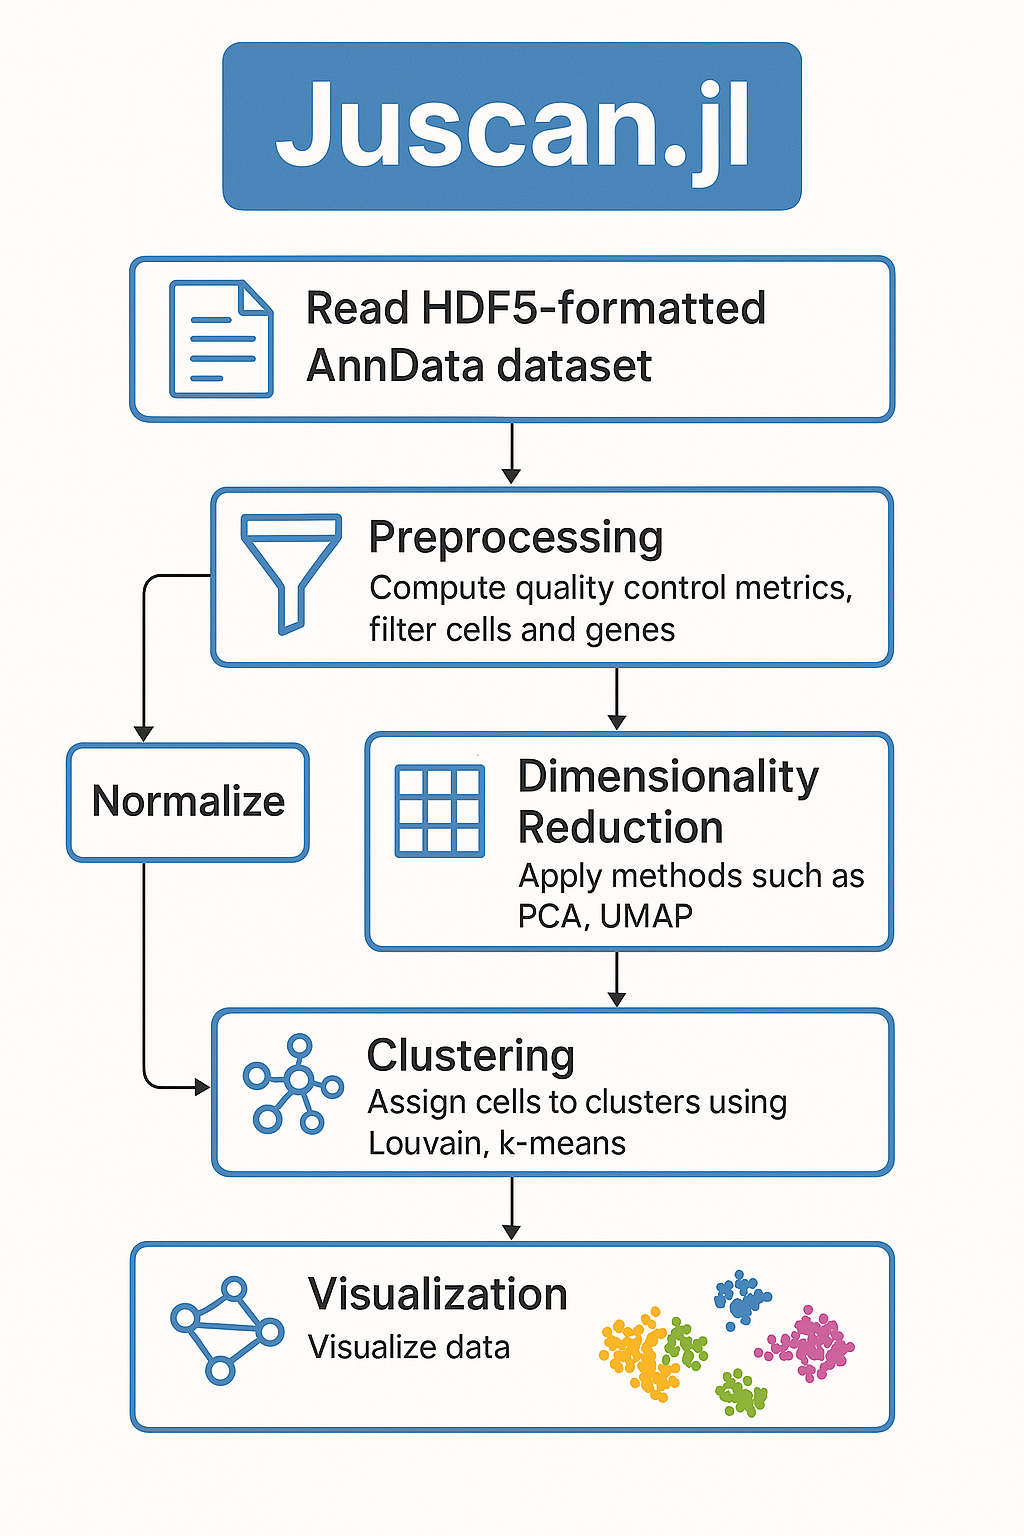
\includegraphics[width=0.4\textwidth]{img/flow_chart.png}
  \caption{Juscan.jl流程图}
  \label{img:flow}
\end{figure}

\subsection{系统模块划分}

如代码\ref{code:文件结构},此平台使用模块化的设计,将不同的功能划分到各自所属的模块中,以提高代码的整洁性、可维护性和扩展能力。

\begin{fancybox}{文件结构}
\addcontentsline{lot}{table}{代码~\thetcbcounter: 文件结构}
\begin{lstlisting}[numbers=none]
  Juscan.jl/
  ├── src/
  │   ├── preprocessing/
  │   │   ├── filter.jl                   # filter cells and genes
  │   │   ├── normalization.jl            # data normalization methods
  │   │   ├── pp.jl                       # preprocessing module
  │   │   ├── qc.jl                       # quality control methods
  │   │   └── utils.jl
  │   ├── tools/
  │   │   ├── cluster.jl                  # clustering methods
  │   │   ├── hvg.jl                      # highly variable genes
  │   │   ├── louvain.jl                  # louvain clustering
  │   │   ├── modularityClustering.jl     # modularity clustering
  │   │   ├── pca.jl                      # dimensionality reduction
  │   │   ├── snn.jl                      # SNN neighbour
  │   │   └── tl.jl                       # tools 
  │   ├── plots/
  │   │   ├── colors.jl
  │   │   ├── pl.jl
  │   │   └── plots.jl
  │   ├── Juscan.jl                       # Main module file
  │   ├── anndata.jl                      # anndata utilities
  │   └── utils.jl
  ├── docs/                               # documentation directory
  ├── test/                               # unit test directory
  ├── LICENSE
  ├── Project.toml                        # Julia project files
  └── README.md
\end{lstlisting}
\end{fancybox}

整体的Juscan.jl主要分为文档文件夹,单元测试文件夹,以及源代码文件夹。

源代码文件夹中Juscan.jl为整个项目的主模块,为项目导入需要的依赖库,加载子模块,以及对外暴露API接口。

导入的子模块包括preprocessing, tools, plots, 分别为单细胞的分析提供预处理,主要分析算法与可视化。

本项目由\href{https://github.com/scverse/Muon.jl}{Muon.jl}提供官方的AnnData数据结构, 代码\ref{code:Muon.AnnData}代表了Muon.anndata基本结构。

\section{数据结构}

\begin{fancybox}{Muon.AnnData}
\addcontentsline{lot}{table}{代码~\thetcbcounter: Muon.AnnData}
\begin{lstlisting}[language=julia]
mutable struct AnnData <: AbstractAnnData
  file::Union{HDF5.File, HDF5.Group, Nothing}

  X::Union{AbstractMatrix{<:Number}, Nothing}

  obs::DataFrame
  obs_names::Index{<:AbstractString}

  var::DataFrame
  var_names::Index{<:AbstractString}

  obsm::StrAlignedMapping{Tuple{1 => 1}, AnnData}
  obsp::StrAlignedMapping{Tuple{1 => 1, 2 => 1}, AnnData}

  varm::StrAlignedMapping{Tuple{1 => 2}, AnnData}
  varp::StrAlignedMapping{Tuple{1 => 2, 2 => 2}, AnnData}

  layers::AbstractAlignedMapping{Tuple{1 => 1, 2 => 2}, String}

  uns::Dict{<:AbstractString, <:Any}
end
\end{lstlisting}
\end{fancybox}

\begin{figure}[htbp]
  \centering
  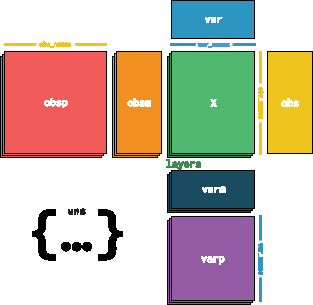
\includegraphics[width=0.5\textwidth]{img/anndata_schema.pdf}
  \caption{anndata数据结构示意图}
  \label{img:anndata}
\end{figure}


但是Muon.jl并没有提供足够多的处理anndata数据结构的方法行为,为了补充这方面的不足,本项目在\lstinline|src/anndata.jl|文件中进行了一些简单的扩充,包括子集化,插入观测与特征数据框,获取与设观测值的各个维度等方法。

\section{数据预处理模块}

\subsection{计算质量控制指标}

为了评估单细胞或多组学数据中的细胞与基因质量,我们实现了一个模块化的质量控制(quality control, QC)指标计算函数 \code{calculate_qc_metrics}。该函数支持从不同表达矩阵源(如主矩阵、原始计数矩阵 \code{adata.raw.X} 或指定的 \code{layer})提取表达数据,并分别计算细胞和基因层面的多种常用 QC 指标。

该函数的调用格式如下:

\begin{fancybox}{Muon.Pp.calculateQcMetrix}
\addcontentsline{lot}{table}{代码~\thetcbcounter: Muon.Pp.calculate\_qc\_metrix}
\begin{lstlisting}[language=julia]
calculate_qc_metrics(
  adata;
  expr_type="counts",
  var_type="genes",
  qc_vars=String[], 
  percent_top=[50, 100, 200, 500],
  layer=nothing,
  use_raw=false, 
  use_log1p=true,
  parallel=nothing
)::Tuple{DataFrame, DataFrame}
\end{lstlisting}
\end{fancybox}

在细胞维度上,函数会统计每个细胞中被检测到的特征数量、总表达量、log 转换后的表达水平、以及前若干高表达基因(如前 50、100、200 和 500 个)所占的表达比例。此外,用户可通过 \code{qc_vars} 参数指定一组具有特殊生物学意义的基因类别(如线粒体基因、核糖体基因等),函数将进一步评估这些类别基因在各细胞中的表达总量和比例。

在基因维度上,函数则计算每个基因在细胞群体中的检测频率、平均表达水平、零表达比例(dropout rate)以及总表达量等指标。这些指标可用于后续的基因过滤与特征选择。

函数 \code{calculate_qc_metrics} 返回两个 \code{DataFrame} 对象,分别包含细胞与基因层面的 QC 指标;而对应的 \code{calculate_qc_metrics!} 则为原地版本,直接将计算结果存储于 \code{adata.obs} 与 \code{adata.var} 字段中,便于与后续分析模块协同使用。

为支持灵活的数据接口设计,该模块还实现了表达矩阵的抽象选择函数 \code{_choose_mtx_rep},并对核心 QC 计算逻辑进行了进一步拆分,分别实现了用于细胞维度的 \code{describe_obs}/\code{describe_obs!} 和基因维度的 \code{describe_var}/\code{describe_var!}。其中,top-n 表达占比的计算由辅助函数 \code{top_segment_proportions} 实现。

该模块参考了 Scanpy 与 Seurat 的 QC 实践流程,并结合 Julia 类型系统设计了更高的通用性与可组合性,便于集成到多模态数据分析管线中。

\subsection{过滤}

在质量控制指标计算之后,我们进一步对数据进行细胞与基因的过滤,以剔除潜在的低质量条目,减少技术噪声对下游分析的干扰。本研究实现了一套通用的过滤函数,支持以总表达量、检测到的基因数(或细胞数)为阈值,灵活筛选细胞或基因,如代码\ref{code:Muon.Pp.filter}。

\begin{fancybox}{Muon.Pp.filter}
\addcontentsline{lot}{table}{代码~\thetcbcounter: Muon.Pp.filter}
\begin{lstlisting}[language=julia]
filter_cells!(
  data::Muon.AnnData;
  min_counts=nothing, min_genes=nothing,
  max_counts=nothing, max_genes=nothing
)::Nothing
filter_genes!(
  data::Muon.AnnData;
  min_counts=nothing, min_cells=nothing,
  max_counts=nothing, max_cells=nothing
)::Nothing
\end{lstlisting}
\end{fancybox}

细胞过滤函数 \code{filter_cells} 支持以下常用策略:

  \begin{itemize}
    \item 最小/最大总表达量(\code{min_counts}, \code{max_counts})
    \item 最小/最大检测基因数(\code{min_genes}, \code{max_genes})
    \item 可选择返回布尔向量(用于掩码子集)或过滤后的新对象(通过设置 \code{copy=true})
    \item 同时提供 \code{filter_cells!} 实现原地修改。
  \end{itemize}

类似地,基因过滤函数 \code{filter_genes} 支持以以下标准筛选:

  \begin{itemize}
    \item 被表达的细胞数量阈值(\code{min_cells}, \code{max_cells})
    \item 总表达量阈值(\code{min_counts}, \code{max_counts})
    \item 同样支持返回掩码或直接修改 \code{AnnData} 对象
  \end{itemize}

为确保操作语义明确,所有函数均要求每次仅传入一个过滤标准,以避免混淆。被筛选出的条目数量将在控制台输出日志,便于用户了解过滤效果。

该模块基于 Juscan.subset\_adata! 接口统一实现子集化操作,保证了代码的可维护性与高一致性,可无缝集成至数据预处理工作流中。

\subsection{归一化}


为消除不同细胞测序深度(即总 UMI 数)差异所带来的偏倚,我们实现了一个可扩展的总表达量归一化函数 \code{normalize_total},用于将每个细胞的表达矩阵缩放至统一的目标总量。该方法类似于 Scanpy 中的 \code{normalize_total} 或 Seurat 中的 \code{NormalizeData},但更具灵活性与模块化。

\begin{fancybox}{Muon.Pp.normalize}
\addcontentsline{lot}{table}{代码~\thetcbcounter: Muon.Pp.normalize}
\begin{lstlisting}
normalize_total(
    adata::AnnData;
    target_sum::Union{Real, Nothing}=nothing,
    exclude_highly_expressed::Bool=false,
    max_fraction::Float64=0.05,
    key_added::Union{String, Nothing}=nothing,
    layer::Union{String, Nothing}=nothing,
    layers::Union{String, Vector{String}, Nothing}=nothing,
    layer_norm::Union{String, Nothing}=nothing,
    copy::Bool=false
)::Union{AnnData, Dict{String, Any}}
normalize_total!(
    adata::AnnData;
    target_sum::Union{Real, Nothing}=nothing,
    exclude_highly_expressed::Bool=false,
    max_fraction::Float64=0.05,
    key_added::Union{String, Nothing}=nothing,
    layer::Union{String, Nothing}=nothing,
    layers::Union{String, Vector{String}, Nothing}=nothing
)::Nothing
\end{lstlisting}
\end{fancybox}

该函数通过计算每个细胞的总表达量(按行求和)作为归一化因子,并将表达矩阵按比例缩放,从而实现标准化。若未指定目标值(\code{target_sum}),则默认将每个细胞归一化至群体中位总表达量。此外,函数允许用户通过参数 \code{exclude_highly_expressed} 排除在某些细胞中高度表达的基因(如线粒体或核糖体基因),避免其对归一化因子的主导效应。

我们提供了两种版本的归一化函数:

    \code{normalize_total}:返回归一化后的新对象或结果字典;

    \code{normalize_total!}:原地(in-place)修改原始数据结构,节省内存。

这两个函数均支持对单个 \code{layer} 或多个 \code{layers} 进行归一化操作,并可通过参数 \code{layer_norm} 控制不同层归一化的参考因子。此外,归一化因子也可通过 \code{key_added} 参数保存至 \code{adata.obs} 中,用于后续批量分析或可视化。

值得注意的是,对于表达全为零的细胞,函数会发出警告提示。我们建议在归一化之前结合质量控制结果,先剔除此类无信息细胞。

\section{工具模块}

\subsection{高可变基因}

在单细胞 RNA 测序分析中,高变异基因(highly variable genes, HVGs)的识别对于后续的降维、聚类与轨迹推断等分析具有重要意义。为此,我们基于 Seurat v3 的策略,在 Julia 中实现了一套高变基因筛选模块 \code{highly_variable_genes},该方法兼容批次(batch-aware)处理,适用于多样本或多组学场景下的高变基因筛选。

该方法首先对每个批次独立计算每个基因的平均表达量与方差,并通过 LOESS 回归(局部加权多项式拟合)建模均值-方差关系,获得期望方差。随后,对原始方差进行校正,计算归一化后的方差作为变异性的衡量指标。对于跨多个批次的分析,方法进一步对各批次筛选结果进行合并,通过多批次中位排名的方式选出最终的一组 HVGs,保证其在多个批次中稳定地表现出高变异性。

我们实现了以下三类函数接口:

    % \code{highly_variable_genes}:返回 HVG 信息的 \code{DataFrame},不修改原始数据;
    % \code{highly_variable_genes!}:原地执行 HVG 计算,并将结果添加到 \code{adata.var};
    % \code{subset_to_hvg!}:在执行 HVG 筛选后,将数据集子集化,仅保留被识别为高变异的基因。
\begin{fancybox}{Muon.Tl.hvg}
\addcontentsline{lot}{table}{代码~\thetcbcounter: Muon.Tl.highly\_variable\_genes}
\begin{lstlisting}
subset_to_hvg!(adata::AnnData;
  layer::Union{String,Nothing} = nothing,
  n_top_genes::Int=2000,
  batch_key::Union{String,Nothing} = nothing,
  span::Float64=0.3,
  verbose::Bool=true
)
highly_variable_genes(adata::AnnData;
  layer::Union{String,Nothing} = nothing,
  n_top_genes::Int=2000,
  batch_key::Union{String,Nothing} = nothing,
  span::Float64=0.3
)
highly_variable_genes!(adata::AnnData;
  layer::Union{String,Nothing} = nothing,
  n_top_genes::Int=2000,
  batch_key::Union{String,Nothing} = nothing,
  span::Float64=0.3,
  replace_hvgs::Bool=true,
  verbose::Bool=false
)
\end{lstlisting}
\end{fancybox}

函数输出包括每个基因的均值、方差、归一化方差、在多个批次中的高变频次,以及最终的变异性排名。若数据中已有 HVG 注释,用户可选择是否替换(\code{replace_hvgs=true})。

\subsection{降维}

我们首先实现了 \code{log_transform!} 与 \code{logp1_transform!} 函数,用于对数据执行 $\log(x + \varepsilon)$ 或 $\log(1 + x)$ 变换,以增强表达量在低值区间的分布分辨能力。默认会将结果保存至新的数据层,便于复用与回溯。此外,函数 \code{standardize} 与 \code{prcomps} 封装了标准化与主成分提取过程,提供更底层的控制接口。

\subsubsection{(1)pca}

函数 \code{pca!} 实现了对 \code{AnnData} 对象中指定数据层的 PCA 计算,并将结果存储于 \code{adata.obsm["PCA"]} 中,供后续分析调用。该函数支持自动寻找合适的输入表达矩阵:若未提供目标数据层,则会依次查找是否存在经过对数转换的表达矩阵(\code{"log_transformed"})或归一化数据层(\code{"normalized"});若均不存在,则自动执行归一化与对数转换流程。

\begin{fancybox}{Muon.Tl.pca}
\addcontentsline{lot}{table}{代码~\thetcbcounter: Muon.Tl.pca}
\begin{lstlisting}
pca!(
  adata::Muon.AnnData;
  layer::String="log_transformed",
  n_pcs::Int=1000,
  verbose::Bool=true
)
\end{lstlisting}
\end{fancybox}

为确保主成分数量的合理性,函数会根据数据矩阵的维度自动调整主成分数量(\code{n_pcs}),避免维度溢出问题。计算过程采用稠密矩阵的奇异值分解(SVD)或稀疏矩阵的截断 SVD(TSVD),以兼容不同规模数据。

\subsubsection{(2)umap}

\begin{fancybox}{Muon.Tl.umap}
\addcontentsline{lot}{table}{代码~\thetcbcounter: Muon.Tl.umap}
\begin{lstlisting}
umap!(
  adata::Muon.AnnData;
  layer::String="log_transformed",
  use_pca_init::Bool=false,
  n_pcs::Int=100,
  verbose::Bool=true,
  kwargs...
)
\end{lstlisting}
\end{fancybox}

函数 \code{umap!} 用于计算数据的 UMAP 嵌入,并将结果包括嵌入坐标、最近邻索引、距离矩阵与模糊邻接图分别存入 \code{adata.obsm} 与 \code{adata.obsp} 中。该函数支持两种初始化方式:

\begin{itemize}
  \item 直接嵌入:使用指定数据层或自动生成的对数转换数据
  \item PCA 初始化:通过设置 \code{use_pca_init=true},先执行 PCA 作为初始嵌入向量
\end{itemize}

UMAP本身使用\code{UMAP.jl}实现,默认基于余弦距离构建邻接图,并可通过传入关键字参数(如 \code{n_neighbors}, \code{min_dist} 等)实现参数化控制。

\subsection{聚类}

聚类分析是单细胞数据中识别细胞亚群结构的关键步骤。此部分代码部分参考\code{ASCT.jl}的实现方法\upcite{Yang2023.12.27.573479}, 对\code{Muon:Ammdata}数据结构进行两类聚类方法:图结构驱动的模块度聚类(modularity clustering)与基于中心点的 KMedoids 聚类(近似 KMeans),构成了双路径的细胞聚类框架。为了便于用户在不同分析阶段调用聚类方法,我们提供了统一接口 clustering!,支持多种参数配置与算法选择。

\begin{fancybox}{Muon.Tl.Clustering}
\addcontentsline{lot}{table}{代码~\thetcbcounter: Juscan.Tl.Clustering}
  \begin{lstlisting}
function clustering!(
  data::Muon.AnnData;
  method::AbstractString="mc",
  reduction::Union{AbstractString, Symbol}=:auto,
  use_pca::Union{AbstractString, Integer}="pca_cut",
  # n_pcs::Union{Integer, AbstractString}=5,
  tree_K::Integer=20,
  resolution::Union{Symbol, Real, AbstractRange}=:auto,
  cluster_K::Union{Nothing, Integer}=nothing,
  cluster_K_max::Union{Nothing, Integer}=30,
  dist::AbstractString="Euclidean",
  network::AbstractString="SNN",
  random_starts_number::Integer=10,
  iter_number::Integer=10,
  prune::AbstractFloat=1 / 15,
  seed::Integer=-1,
)
  \end{lstlisting}
\end{fancybox}

对\code{AnnData}对象执行聚类分析,结果会自动保存在\code{adata.obs}中。该函数根据参数\code{method}选择不同的聚类策略。

\textbf{a.~基于模块度的图聚类(modularity clustering)}

该方法通过构建细胞的共享最近邻图(Shared Nearest Neighbor, SNN),并以最大化模块度(modularity)为目标,对细胞图进行社团划分。方法流程如下:

\begin{enumerate}
  \item 图构建:在降维空间(如 PCA)中,使用 KD 树加速寻找每个细胞的 $K$ 个近邻,构建 KNN 或 SNN 图。SNN 图定义如下:

\begin{equation}
  \text{SNN}_{ij} = |\mathcal{N}_i \cap \mathcal{N}_j| / K
\end{equation}

其中 $\mathcal{N}_i$ 表示细胞 $i$ 的邻居集合。

\item 图稀疏化与剪枝:通过阈值参数 $\alpha \in (0, 1]$ 对图进行稀疏化,仅保留重叠度高的邻接关系,以提高模块度检测的稳定性。

\item 模块度优化聚类:通过 Louvain 或 Leiden 等算法,在图中最大化以下模块度函数:

\begin{equation}
Q = \frac{1}{2m} \sum_{i,j} \left( A_{ij} - \gamma \frac{k_i k_j}{2m} \right) \delta(c_i, c_j)
\end{equation}

其中 $A_{ij}$ 为图邻接矩阵,$k_i$ 为节点度,$\gamma$ 为分辨率参数,$\delta$ 为 Kronecker delta。我们支持不同的 $\gamma$ 参数进行多分辨率扫描,自动推荐最优分辨率。

\end{enumerate}

\textbf{b.~基于KMedoids的中心点聚类(k-medoids clustering)}

KMedoids 聚类是一种鲁棒于异常值的变体,相较于 KMeans 选择“簇中心”,KMedoids 选择实际数据点作为中心。我们实现如下自动聚类过程:

\begin{enumerate}
  \item 距离计算:用户可选择多种距离度量,如欧氏距离、余弦距离、相关距离等,在降维空间中计算细胞间距离矩阵。

  \item 自动选择簇数 $K$:

  \begin{itemize}
    \item 计算多个 $K$ 值下的聚类结果(并行加速);
    \item 对每个聚类结果,计算 silhouette 系数 $\bar{s}$ 与标准差;
    \item 同时评估总成本的肘部法则(elbow method);
    \item 综合两个指标,自动选择最优 $K$ 值:
  \end{itemize}

\end{enumerate}

\begin{equation}
K^* = \arg\max_K \left( \text{silhouette score} - \text{total cost deviation} \right)
\end{equation}

\section{可视化模块}

单细胞组学分析常涉及高维数据的降维、聚类和分类结果,为了更好地呈现这些复杂结构,我们在 \code{Juscan.Plots} 中实现了一套基于 \code{CairoMakie} 的绘图模块,涵盖多种用于探索性分析与结果展示的图形函数。该模块强调高可配置性、视觉一致性与图像质量,便于科研报告与论文作图。

\subsection{调色机制与主题色板}

我们设计了一套模块化的调色系统,通过 \code{get_palette} 和 \code{get_continuous_colormap} 接口,提供一系列离散与连续的调色方案,支持自动扩展与下采样。其中,离散色板如 \code{"friendly"}、\code{"apple"}、\code{"rainbow"} 等适用于类别标签着色,而连续色带则集成自 \code{ColorSchemes.jl},可用于表达量、主成分值等数值信息的可视化。所有色板均通过自定义函数实现扩展与裁剪策略,确保图形风格在多图展示中保持一致。

\subsection{可视化函数接口}

模块当前提供以下核心函数:

\begin{itemize} \item \code{violin}:绘制提琴图,展示多个观测变量(如基因表达、细胞指标)的分布,支持点抖动(jitter)与多子图并排布局。 \item \code{scatter}:绘制二维散点图,支持根据第三变量进行着色(如根据表达量、UMAP/PCA位置等变量上色)。 \item \code{hvg_scatter}:用于展示高变异基因的筛选结果,通过平均表达与变异度关系图突出高变基因在全体中的位置。 \item \code{plot_variance_ratio}:绘制 PCA 主成分的方差解释比例图,支持对前若干主成分进行可视化,并自动标注前 5 个 PC。 \item \code{plot_umap}:绘制 UMAP 降维嵌入图,支持按照类别标签上色,自动生成图例并匹配色板风格。 \end{itemize}

\subsubsection{(1) violin:分布可视化}

该函数支持绘制多个变量在样本中的表达分布,可用于细胞质控指标(如总 UMI 数、线粒体比例)的展示。用户可指定色板名与透明度参数,自动匹配子图数量与调色方案。此外还可设置点抖动强度与保存图像路径:

\begin{fancybox}{Juscan.Plots.violin} 
  \addcontentsline{lot}{table}{代码~\thetcbcounter: Muon.Pl.violin}
  \begin{lstlisting} 
violin(
  adata::AnnData,
  keys::Union{String, Vector{String}};
  width::Real=600,
  height::Real=400,
  jitter::Union{Bool, Real}=0.5, dot_size::Real=2,
  title::String="violin plot",
  palette_name::String="friendly",
  fill_alpha::Real=1.0, 
  savefig::Union{Bool, String}=false
) 
  \end{lstlisting} 
\end{fancybox}

\subsubsection{(2) hvg\_scatter:高变基因展示}

为辅助用户评估 HVG 的筛选结果,我们实现了 \code{hvg_scatter} 函数,绘制均值-方差与归一化方差的二维图。灰色表示非 HVG 基因,黑色点表示已筛选出的 HVGs,有助于观察其在全体中的分布位置。

\subsubsection{(3) plot\_umap:嵌入可视化}

该函数根据 \code{adata.obsm} 中的 UMAP 坐标绘图,并根据 \code{adata.obs} 中的分类变量进行着色。支持自定义调色板、图形尺寸与图像保存路径:

\begin{fancybox}{Juscan.Plots.plot umap}
  \addcontentsline{lot}{table}{代码~\thetcbcounter: Muon.Pl.plot\_umap}
  \begin{lstlisting} 
plot_umap(
  adata;
  color_by::String="clusters_latest",
  key="umap",
  palette_name::String="rainbow",
  savefig::Union{Bool, String}=false
) 
  \end{lstlisting} 
\end{fancybox}

\subsubsection{(4) scatter 与 plot\_variance\_ratio}

除标准二维散点图外,我们也实现了用于主成分方差比分析的函数 \code{plot_variance_ratio}。其通过绘制 log 方差比图,帮助用户直观判断 PCA 的有效维度。


\chapter{实验流程与方法}
\section{实验流程}

\begin{figure}[H]
  \centering
  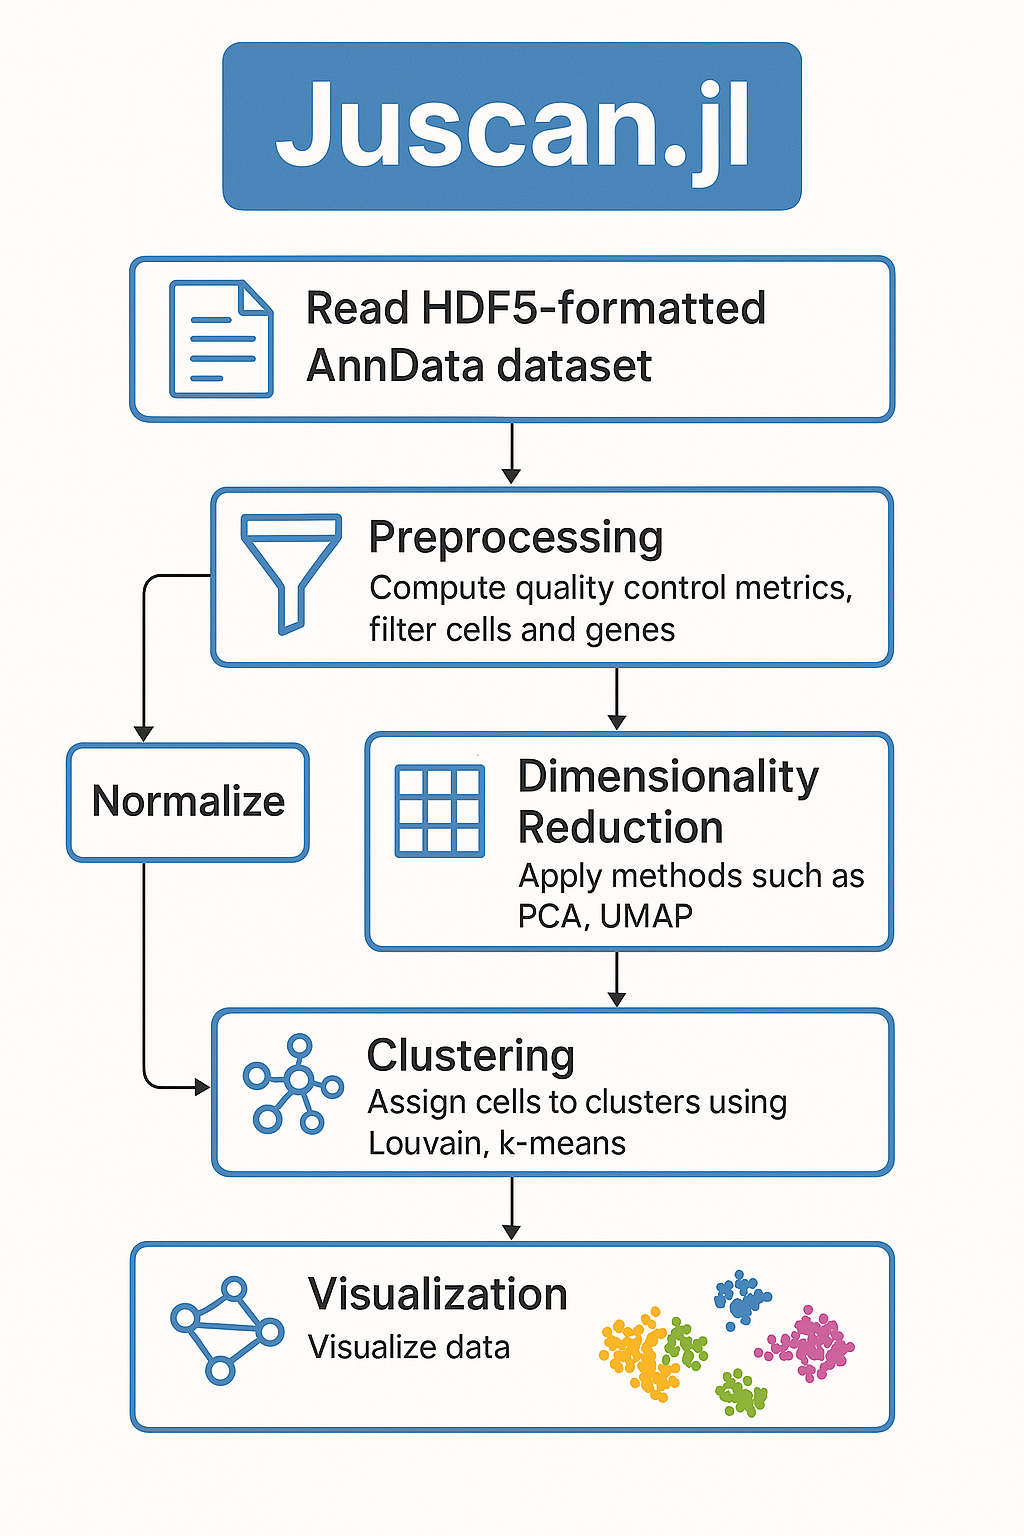
\includegraphics[width=0.57\textwidth]{img/flow_chart.png}
  \caption{实验流程}
  \label{fig:flow_chart}
\end{figure}

\section{实验方法}

\subsection{扩增插入基因}

\textbf{一、引物设计}

\begin{enumerate}[itemsep=0.1em]
\item 使用高质量的模板。
\item 勿使用dUTP和带有尿嘧啶的引物和模板。
\item 如实验需要,可适当提高Phanta酶的使用量,但50ul体系内酶量建议不要超过2ul。
\item Phanta酶具有较强的校对活性。因此,如扩增产物需要进行TA克隆,加之前必须进行DNA纯化。
\item 为了防止Phanta酶的校对活性降解引物,在配制反应体系时请最后加入聚合酶。
\item 引物设计
\begin{enumerate}[label={(\arabic*)}, itemsep=0.1em]
  \item 引物3端最后一个碱基最好为G或者C;
  \item 引物3端最后8个碱基应避免出现连续错配;
  \item 引物3端应避免出现发夹结构;
  \item 正向引物和反向引物的Tm值相差不超过1℃为佳,Tm值调整至55~65℃为佳;
  \item 引物额外附加序列,即与模板非配对序列,不应参与引物Tm值计算
  \item 引物的GC含量控制在40\%-60\%之间;
  \item 引物A、G、C、T整体分布要尽量均匀,避免使用GC或者AT含量高的区域;
  \item 引物内部或者两条引物之间避免有5个碱基以上的互补序列,两条引物的3端避免有3个碱基以上的互补序列;
  \item 引物设计完毕请使用NCBI BLAST功能检索引物特异性,以避免非特异性扩增产生。
\end{enumerate}
\end{enumerate}

\textbf{二、PCR}(Panta酶反应体系,从全基因组中PCR结束之后需要做一步消化。要注意全程在冰上操作,加的体积从大到小)

\begin{longtable}{cc}
  \caption{PCR 反应体系} \\
  \toprule
  \textbf{组分} & \textbf{体积} \\
  \midrule

  ddH$_2$O & 17~$\mu$l(加到 50~$\mu$l) \\
  2$\times$Buffer & 25~$\mu$l \\
  dNTP & 1~$\mu$l \\
  上、下游引物(分开加) & 2~$\mu$l \\
  酶 & 1~$\mu$l \\
  模板 DNA & 2~$\mu$l \\

  \bottomrule
\end{longtable}


\begin{longtable}{ccc}
  \caption{PCR 反应条件} \\
  \toprule
  \textbf{步骤} & \textbf{时间} & \textbf{温度} \\
  \midrule
  \endfirsthead

  \multicolumn{3}{l}{\textit{续表:PCR 反应条件}} \\
  \toprule
  \textbf{步骤} & \textbf{时间} & \textbf{温度} \\
  \midrule
  \endhead

  \bottomrule
  \multicolumn{3}{r}{\textit{表格接下页}} \\
  \endfoot

  \bottomrule
  \endlastfoot

  预变性 & 3 min & 95$^\circ$C \\
  变性   & 15 sec & 95$^\circ$C \\
  退火   & 15 sec & 60$^\circ$C(根据引物 Tm 值调整) \\
  延伸   & 150 sec(根据 bp 长度调整) & 72$^\circ$C \\
  彻底延伸 & 5 min & 72$^\circ$C \\

\end{longtable}

\textbf{三.跑胶}

\begin{enumerate}[itemsep=0.1em]
  \item 安仪器,根据要跑胶的基因数目的具体情况计算要用到的梳子种类和皿的种类。
  \item 加溶剂,两次煮沸,在侧面冷水下冲洗到$50^\circ\text{C}$。
  \item 加核酸染料。
  \item 倒胶。
  \item 晾干30min,待胶条凝固冷却成型。
  \item 取梳子。
  \item 转胶条。
  \item 加基因和marker。
  \item 电压150V,电流400A,跑胶。
\end{enumerate}

\textbf{四.胶回收}

\begin{enumerate}[itemsep=0.1em]
  \item 切胶,置于2.0ml EP管中。切胶要放切胶板,切完的胶扔到红色垃圾袋,管中的胶放在相应的引物旁边,作好引物名称标记。
  \item 加3倍凝胶体积的Buffer MB,$55^\circ\text{C}$水浴加热,直至凝胶全部融化。
  \item 在等待胶溶期间,向离心吸附柱中加入500$\mu$l Buffer BL,静止1min,室温下12,000rpm离心1min,弃收集管中的废液,将离心吸附柱重新放回收集管中。
  \item 待凝胶溶液冷却至室温后,转移到离心吸附柱内,静置1min,室温下12,000rpm离心1min。
  \item 弃除收集管中的废液,将离心吸附柱重新插回收集管中。
  \item 加入600$\mu$l Buffer MW于离心吸附柱中,室温下12,000rpm离心30s,弃除收集管中的废液,将离心吸附柱重新插回收集管中。
  \item 重复操作步骤6。
  \item 室温下12,000rpm空离2min,弃除收集管。
  \item 将吸附柱置于1.5ml离心管中,加入50$\mu$l\~100$\mu$l至吸附柱中央,室温静置1min,12,000rpm离心1min。
  \item 弃去吸附柱,获得的DNA片段可直接用于后续反应或于$-20^\circ\text{C}$长期保存。
\end{enumerate}

\subsection{扩增质粒}

\textbf{一.摇菌(扩增质粒数量)}

\textbf{二.提质粒}

\begin{enumerate}[itemsep=0.3em]
  \item 取摇菌管,4000rpm离心3min。弃去培养基,将摇菌管倒扣于吸水纸上吸尽残液。
  \item 向留有菌体沉淀的摇菌管中加入250$\mu$l Buffer P1,用移液器或涡旋振荡混匀后将其转入1.5ml离心管中。
  \item 向步骤2中加入250$\mu$l Buffer P2,温和地上下颠倒混匀8–10次,使菌体充分裂解。
  \item 向步骤3中加入350$\mu$l Buffer P3,立即温和地上下颠倒8–10次使溶液彻底中和。将混合液加入吸附柱中,12,000rpm离心30–60s,弃废液并将吸附柱重新放回收集管中。
  \item 重复步骤4。
  \item 将吸附柱放入新的1.5ml离心管中,12,000rpm离心2min,以干燥吸附柱,彻底去除残留漂洗液。
  \item 将吸附柱再次置于新的灭菌1.5ml离心管中,加入30$\mu$l无菌水至吸附柱膜中央,室温静置2min,12,000rpm离心1min以洗脱DNA。
  \item 测定质粒DNA浓度,并在离心管上做好标记。
\end{enumerate}

\subsection{构建新的质粒}

\textbf{一、酶切}

\begin{longtable}{cc}
  \caption{酶切体系} \\
  \toprule
  \textbf{组分} & \textbf{用量} \\
  \midrule
  \endfirsthead

  \multicolumn{2}{l}{\textit{续表:酶切体系}} \\
  \toprule
  \textbf{组分} & \textbf{用量} \\
  \midrule
  \endhead

  \bottomrule
  \endfoot

  \bottomrule
  \endlastfoot

  Plasmid & 2~$\mu$g \\
  Enzyme 1 & 1~$\mu$l \\
  Enzyme 2 & 1~$\mu$l \\
  10$\times$酶切 Buffer & 3~$\mu$l \\
  ddH$_2$O & up to 30~$\mu$l \\
  
\end{longtable}

震荡混匀,37$^\circ\text{C}$酶切30min(3000bp酶切30min)

\textbf{二、纯化}(与胶回收的原理和步骤类似)

\textbf{三、连接}

弹管混匀后冰浴30min

\begin{longtable}{cc}
  \caption{连接体系} \\
  \toprule
  \textbf{组分} & \textbf{用量} \\
  \midrule
  \endfirsthead

  \multicolumn{2}{l}{\textit{续表:连接体系}} \\
  \toprule
  \textbf{组分} & \textbf{用量} \\
  \midrule
  \endhead

  \bottomrule
  \endfoot

  \bottomrule
  \endlastfoot

  载体 & 30~ng(3~$\mu$l / 2~$\mu$l) \\
  插入序列 & 50~ng(5~$\mu$l / 6~$\mu$l) \\
  10$\times$酶切 Buffer & 1~$\mu$l \\
  Exo3 & 1~$\mu$l(取 1~$\mu$l 加到 9~$\mu$l 水中,稀释 10 倍后取 1~$\mu$l) \\
\end{longtable}

\textbf{四.转化}

\begin{enumerate}[itemsep=0.1em]
  \item 取感受态细胞放冰上解冻。
  \item 向感受态细胞中加入10$\mu$l连接产物,弹管混匀。
  \item 冰浴10min。
  \item 42$^\circ$\text{C}热激90s。
  \item 冰浴3\~5min。
  \item 在超净台中加入1ml不含抗生素的LB培养基,混匀后于37$^\circ$\text{C}孵育1h。
  \item 5,000rpm离心4min,吸走上清,只留100$\mu$l,吹打重悬后涂布于抗性平板上。
  \item 置于37$^\circ$\text{C}培养10–16h。
  \item 挑取单克隆接种至含抗生素的LA液体培养基中,小摇培养约3h。
\end{enumerate}

\textbf{注意:}需要设置一个阴性对照——酶切后的载体(3$\mu$l,无需添加连接酶),用于判断载体是否被完全切开或发生自我连接。

\subsection{PCR 验证和测序}

\textbf{一、菌液PCR}

\textbf{二、跑胶验证}

\subsection{RNAi 实验}

\begin{enumerate}[itemsep=0.3em]

  \item 第0天:在含抗生素的LB液体培养基中接种含有RNAi质粒的HT115大肠杆菌,于37$^\circ$\text{C}震荡培养12–16小时,以获取最多的活菌。
  
  \item 第一天:
  \begin{enumerate}[label*={(\alph*)}, itemsep=0.3em]
    \item 将菌液1:100稀释至2$\times YT ^+$ 抗生素中,培养至OD$_{595}$ = 0.4;
    \item 加入无菌 IPTG 使终浓度达到0.4mM,在37$^\circ$\text{C}摇床诱导4小时;
    \item 在含抗生素和IPTG的培养条件下继续培养。可直接使用培养液,也可将菌液以2000rpm离心、吸走上清后重悬浓缩细胞,然后播种至RNAi平板上。
  \end{enumerate}
  
  \item 挑选线虫至RNAi平板上,开始RNAi实验。
  
\end{enumerate}

\subsection{Smurf Assy 实验}

\begin{enumerate}[itemsep=0.1em]
  \item 提前一天使用LB培养基摇菌OP50(线虫的食物),于37$^\circ$\text{C}培养12–16小时。使用前将菌液浓缩10倍。
  \item 配制5\% Smurf染液:在浓缩后的菌液中加入0.25g Smurf染料粉末,加入5ml浓缩菌液,涡旋混匀备用。
  \item 用2ml离心管,加入200$\mu$l M9缓冲液,将待处理线虫挑入管中。再加入400$\mu$l步骤2中配制的5\% Smurf染液。
  \item 将混合液放置在20$^\circ$\text{C}水平摇床上,缓慢摇晃3小时。
  \item 使用台式小型离心机离心10s,使线虫沉降至管底。吸去上清,保留约300$\mu$l液体,补加1ml M9,轻轻重悬清洗。重复洗涤多次,直到线虫体表的蓝色染料明显变淡,能透过离心管看到手指为止。最后保留约300$\mu$l液体。
  \item 将洗后的线虫液体,用低吸附枪头滴加在已吹干的NGM平板上,轻轻摇晃,使液体尽可能摊平于平板表面。从该平板中挑取线虫转移到无菌NGM平板(用于拍照)。
  \item 在无菌NGM平板上加入叠氮化钠杀死线虫,排列整齐后进行拍照观察。根据Smurf染料在虫体内的渗透程度,判断线虫肠道屏障的完整性。
\end{enumerate}

\subsection{荧光共聚焦实验}


\begin{enumerate}[itemsep=0.1em]
\item 使用左旋咪唑麻醉线虫,将线虫进行排列(每个RNAi组拍摄大约30条虫子)。
\item 使用488nm波长的荧光通道,拍摄线虫表皮细胞间HMR-1-GFP的点状荧光信号。
\end{enumerate}

\section{小结}

本章节详细描述了从基因扩增到荧光共聚焦实验的完整实验步骤,涵盖了DNA操作,RNAi实验以及线虫屏障相关实验多个环节。整个实验流程设计严谨,步骤清晰,我们的实验确保了每一步操作的准确性和可重复性,为研究基因功能和线虫生物学特性提供了可靠的实验方法。

我们的实验首先从引物设计开始,整个引物设计规则严谨,为了确保后续的一系列实验按部就班开展。在扩增插入基因时,我们使用Phanta酶进行PCR反应, PCR产物会通过跑胶和胶回收进行纯化。接下来是质粒的扩增和提取。我们通过摇菌培养细菌以扩增质粒数量,然后进行质粒提取,最终获得高纯度质粒DNA。在构建新的质粒时,我们首先对质粒进行酶切,酶切后的载体通过纯化去除杂质,然后与插入目的片段进行连接,连接产物又通过转化进入感受态细胞,经过培养后在氨苄板上筛选阳性克隆。为了验证阳性克隆,本实验采用菌液PCR和跑胶验证,以确保插入序列的正确性。

随后我们进行RNAi实验。首先我们在LB培养基中培养HT115菌株,加入IPTG诱导dsRNA表达涂板。然后我们将线虫转移到RNAi平板上进行喂养。Smurf Assay实验用于评估线虫肠道屏障功能,利用浓缩菌液配制5\%的 Smurf染料,对线虫进行染色后通过离心、洗涤和显微镜观察得出线虫肠道屏障损伤程度结果。最后,荧光共聚焦拍摄和判断线虫表皮屏障的受损情况。最后两种判断线虫屏障受损与否的实验结果我们都将用定量软件进行分析,以确保最终的实验结论严谨可靠。


\chapter{实验结果}
%%% 讨论

\section{研究成果总结}

本研究基于 Julia 编程语言成功设计并实现了一个高性能的单细胞数据分析平台 —— Juscan.jl。该平台以 Muon.jl 所提供的 AnnData 数据结构为核心,复刻并优化了 Scanpy 在 Python 生态中的分析流程,完成了从数据质量控制、标准化、高变基因筛选、降维、聚类到可视化的完整管线,构建出一个功能完备、接口友好、计算高效的分析框架。

更重要的是,Juscan.jl 采用模块化设计,具有良好的可扩展性和可维护性,为后续的算法开发和功能拓展提供了坚实的基础。

\section{未来工作展望}


尽管 Juscan.jl 已实现了基础的单细胞分析功能,但作为一个初步探索性的项目,仍存在许多可提升的方向,具体包括以下几个方面:

\begin{enumerate}
\item 多模态数据支持与整合: 当前版本主要面向 scRNA-seq 数据,未来可进一步支持 ATAC-seq、CITE-seq 以及空间转录组等多组学数据,并结合 Canonical Correlation Analysis、WNN等多模态聚类方法,实现更全面的细胞表征。
\item 更多聚类与轨迹推断算法的集成: 目前聚类模块仅支持 Louvain 与 k-medoids,后续可引入 Leiden 算法、基于高斯混合模型(GMM)的聚类方法,甚至构建基于图卷积神经网络(GCN)的聚类与分类器。同时,可引入 pseudotime 轨迹推断模块,满足发育过程建模的需求。
\item 计算性能的进一步优化: 尽管 Julia 语言本身具备极高的运行性能,但本项目中的部分性能瓶颈主要源于代码层面的实现尚不够成熟。例如,部分函数存在数据复制冗余、内存访问不充分优化、缺乏懒计算等问题,影响了整体的执行效率与稳定性。未来可以通过进一步剖析关键函数的瓶颈(如使用 @profile、@btime 等工具)、重构核心逻辑、合理安排内存布局、并结合并行/多线程机制等方式,显著提升 Juscan.jl 的运行效率与工程质量。同时,也可结合 PackageCompiler.jl 生成系统映像,以减少启动与冷启动时的性能损耗,从而带来更流畅的用户体验。
\item 用户交互体验与可视化增强: 当前可视化模块虽已支持 UMAP、提琴图等常规图形,但仍缺乏交互式浏览器支持。可借助 Makie.jl + Genie.jl 或 Pluto.jl 构建 Web 可视化平台,让用户通过图形界面进行数据探索。
\end{enumerate}


\chapter{总结和期望}
本研究以秀丽隐杆线虫为模式生物,深入探讨了组织蛋白酶家族在体内屏障衰老过程  中的作用与机制。通过该实验,我们不仅验证了既往关于 CPR-6 组织蛋白酶的研究结论, 还扩展了组织蛋白酶家族在衰老过程中的功能谱系。我们成功鉴定了 40 种线虫体内组织  蛋白酶同源物,并通过 smurf assy 实验和观察HMR-1蛋白的分布筛选出了能够显著破坏肠 道和表皮屏障完整性的关键基因。这些基因的表达水平与线虫衰老过程中的屏障功能衰退  呈现显著相关性,证实了组织蛋白酶家族通过降解细胞间连接蛋白破坏组织屏障的分子机  制。这一发现为理解衰老相关病理变化提供了新的视角。

但是在进行 RNAi 实验的过程中,我们发现一些基因被敲低之后,线虫的存活率显著 下降,这可能是由于这几种基因是线虫中较为重要的基因。但至于为什么如此重要的基因 依旧会在线虫衰老的过程中破坏线虫的组织屏障,它们在线虫中的具体作用还有待研究。

本次实验为后续工作提供了多个值得深入探索的方向。比如,我们可以进一步探索这  些蛋白酶与其他衰老相关信号通路的交互作用, 这可能揭示更复杂的衰老调控网络。此外, 鉴于线虫 HMR-1 蛋白与人类连接蛋白的同源性,后续研究我们可将发现的靶点转化到哺  乳动物模型中去,为临床应用提供直接依据。

在应用层面,本研究的成果可能成为延缓组织屏障功能衰退、改善老年相关疾病的创 新疗法。同时,结合基因编辑技术和 RNA 干扰疗法,我们有望实现对衰老过程的精准干 预。

最后,实验的成功离不开实验团队成员的协作与创新。我们期待未来能将更多的基础 研究成果转化为临床应用。随着未来研究的深入,组织蛋白酶家族在衰老医学中的潜力将 被进一步挖掘,为人类健康事业开辟新的篇章。


%=================================================================
%论文后部
\backmatter


%=======%
%引入参考文献文件
%=======%
\bibdatabase{bib/database}%bib文件名称 仅修改bib/ 后部分
\printbib
% \nocite{*} %显示数据库中有的,但是正文没有引用的文献

% \Appendix

\Thanks


相聚于秋,离别在夏,我的大学生活即将落幕。总觉得来日方长,毕业遥遥可及,终于也
到我执笔于此。以为谈及这四年我会行云流水滔滔不绝,可真到下笔时,却只有百感交集。回
望漫漫求学路,并非皆是坦途,但一路前行,一路成长,无论喜悦还是悲伤,所有经历,于我
都是生命的馈赠,所有相遇,于我都是独家的珍宝。这四年来目光所及之处,皆是回忆,我度
过了人生中最青春的年华。万般不舍,心怀感激。 

涓涓恩师情,深深印于心。所谓大学者,非谓有大楼之谓也,有大师之谓也。我要向大学
期间遇到的所有课程教师以及辅导员老师表达我的感谢。任课老师的课程有趣而充实,让我在
大学期间受益匪浅,我从他们非凡的专业知识和各个领域独特的见解中获得的视野将对我未来
的生活和事业具有永恒的意义。辅导员老师的悉心照顾让我在学习上没有了后顾之忧。从知识
到校园生活,让我从一张小白纸逐渐变成了写满知识的书本。 

家人之爱,永记于心。感谢父母二十多年来的悉心培养,感谢父母一直在背后默默支持我
,正是因为你们的支持和付出,才能让我圆满的完成求学之路。失意时给予我鼓励,任性
时给予我宽容,难过时耐心听我吐露心声,你们是我前进路上最大的底气,唯有万般努力
才能成为你们的骄傲,你们永远平安、健康、快乐是我最大的心愿。
非常感谢我的朋友们,我可爱的室友们,感恩相遇,有你们的存在使我这四年并不枯燥,感恩知己,我们一起努力,一起进步,虽然最终我们都会天各一方,但是希望你们能够前程似锦,以梦为马,不负韶华。能够陪伴在我身边的朋友们,希望你们无论之后是在哪里生活、哪里工作,我们也许很难见面,但是唯有爱意不减。

最后我要特别感谢我的指导老师沈义栋老师和金卫林老师,以及我的班主任,张文华老师。桃李不言,这三位老师有着严谨的教学态度,严密的逻辑思维,丰富的学科知识,以及负责任的工作态度,让我在学习和做人方面都受益匪浅。在整个论文的定题、修改过程中也少不了他们的细心审查。我将牢记老师的教诲,不管是对于这个课题,还是对于做人的态度,我将奋力拼搏,修改错误,超越之前的自己。

道阻且长,行则将至。最后,我想感谢我自己。你走的很慢但一直前行;你真诚待人,也被人真诚相待。希望在未来,仍对世界保持好奇心,满怀期待地去热爱生活,砖一瓦不断建立自己的内心秩序,寻找自治的生活方式。我将带着春天的印记远航,尽情播撒梦想的种子,去启山去躬耕,去摇撸开拓,让夏无尽,让秋丰盈,让此生硕硕

\Grade

\end{document}
